% Enable warnings about problematic code
\RequirePackage[l2tabu, orthodox]{nag}

\documentclass{WeSTassignment}

% The lecture title, e.g. "Web Information Retrieval".
\lecture{Introduction to Web Science}
% The names of the lecturer and the instructor(s)
\author{%
  Prof. Dr.~Steffen~Staab\\{\normalsize\mailto{staab@uni-koblenz.de}} \and
%   Ren{\'e}~Pickhardt\\{\normalsize\mailto{rpickhardt@uni-koblenz.de}} \and
   Korok~Sengupta\\{\normalsize\mailto{koroksengupta@uni-koblenz.de}} \and 
    Jun~Sun\\{\normalsize\mailto{junsun@uni-koblenz.de}}
}
% Assignment number.
\assignmentnumber{IV}
% Institute of lecture.
\institute{%
  Institute of Web Science and Technologies\\%
  Department of Computer Science\\%
  University of Koblenz-Landau%
}
% Date until students should submit their solutions.
\datesubmission{November 17, 2017, 11:00 a.m.}
% Date on which the assignments will be discussed in the tutorial.
\datetutorial{November 24, 2017, 12:00 p.m.}

% Specify bib file location.
\addbibresource{bibliography.bib}

% For left aligned centerd boxes
% see http://tex.stackexchange.com/a/25591/75225
\usepackage{varwidth}
\usepackage{amsmath}
% ==============================================================================
% Document

\begin{document}

\maketitle
This assignment focuses on the topics of 1) \textbf{Hello World}, 2) \textbf{Dynamic Web Content}.

For all the assignment questions that require you to write code, make sure to include the code in the answer sheet, along with a separate Python file. If you generate a plot from your Python script, please add them in the answer sheet.\\ \\ 




%Please mention your team Names here: 
Team Name: XXXX


\section{Hello World \hfill (10 points)}
Your task is to print ``Hello, World!'' on the screen.

\subsection*{Solution}
%solution-start
\subsubsection*{hello\_world.py}
\lstinputlisting[language=Python, breaklines=true]{hello_world.py}
%solution-end
%-------------------------------------------------------------------------------

\section{Dynamic Web Content (15 points)}

You are provided with \texttt{DynamicWeb.zip} that contains a simple HTTP web server that we have designed for you. It has a simple HTTP registration page (\texttt{localhost:8080/form}) that asks you to enter the first name and email ID to register.\\

Your task is to write a python script that automates the process of registering. 

The \texttt{DynamicWeb.zip} contains \texttt{contacts.txt} that has the different names and email IDs that you need to register automatically through your script. (4 points)

In the the \texttt{template} folder, you will find an html form whose actions you need to automate through your script. The script should look for error messages if the entry that you are trying to register is already in the system or not. If no error message, your entry gets stored in the server. The script should save all the responses from the server and count the number of successful and unsuccessful attempts to register. (5 points)

\begin{enumerate}
\item Please provide a graphical representation of the successful and unsuccessful attempts of registering in a single graph. (2.5 points)
\item Every time you get a response from the server, within it you will also receive the number of elements in the list (on the server). Save the number of list elements you receive after every response(in a file, local to the directory you run your code from), and plot the changes. (3.5 points)
\end{enumerate}

\textbf{Requirements}
\begin{enumerate}
\item You will need to install the \texttt{lpthw.web}\footnote{Use \texttt{pip install lpthw.web} to install the \texttt{lpthw.web} module used for the server. \\For python 3, use \texttt{pip3 install web.py==0.40.dev0}} library in order to run the server.
\item In order to run the server it is necessary to run the \texttt{python bin/app.py} command (\textbf{from the directory that contains the bin directory}).

\end{enumerate}


You may use \texttt{requests} library if required along with \texttt{matplotlib}. 
Please keep in mind that every time you restart the server, the server starts fresh.  
\subsection*{Solution}
%solution-start
\begin{verbatim}

import requests # This can also be eliminated with a simple function.
import matplotlib.pyplot as plt


def send_request(url,data):
    r = requests.post(url, data)
    return r.status_code, r.text

#Contents of contacts.txt
credentials_list = [
    ["Peter", "pete@gmail.com"],
    ["Korok", "korok@yahoo.com"],
    ["Stefan", "stef@gmail.com"],
    ["Lara", "lara@yahoo.com"],
    ["Jun", "jun@gmail.com"],
    ["Igor", "igor@uni-koblenz.com"],
    ["Claudia", "claudia@gmail.com"],
    ["Ivana", "ivana@airbnb.com"],
    ["Husam", "sam@gmail.com"],
    ["Rajesh", "raj@gmail.com"],
]

url = "http://localhost:8080/form"
def status_codes_from_server(url, credentials_list):
    status_codes = []
    txt = []
    for cred in credentials_list:
        data = {"name":cred[0],"email":cred[1]}
        status, text = send_request(url, data)
        status_codes.append(status)
        txt.append(text)
    return status_codes, txt 

def get_unique_codes(code_list):
    codes = []
    for code in code_list:
        if code not in codes:
            codes.append(code)
    return codes
    
def count_codes(code_list):
    codes = {}
    for i in code_list:
        if i not in codes:
            codes[i] = 1
        else:
            codes[i] += 1 
    return codes

def record_list_size(text_list):
    list_size = []
    for i in text_list:
        list_size.append(int(i.split('<em style="color: green; 
                         font-size: 2em;">')[1].split("<")[0]))
    return list_size


code_list, text_list = status_codes_from_server(url, credentials_list)
print(code_list)
print(text_list)
unique_codes = get_unique_codes(code_list)
print(unique_codes)
count_codes = count_codes(code_list)
print(count_codes)


list_size = record_list_size(text_list)

plt.title('List size timeline')
plt.xlabel('number of responses')
plt.ylabel('num of list items')
plt.plot(list_size)
plt.show()


def plot_bar(count_codes, title, xlabel, ylabel):
    d = count_codes
    plt.bar(range(len(d)), d.values(), align="center")
    plt.xticks(range(len(d)), list(d.keys()))
    plt.title(title)
    plt.xlabel(xlabel)
    plt.ylabel(ylabel)
    plt.show()

def error_success_count(text_list):
    count = {}
    for i in range(0,len(text_list)):
        x = text_list[i].split("<p>")[1].split("!")[0]
        if x not in count:
            count[x] = 1
        else:
            count[x] += 1
    return count

error_sucess = error_success_count(text_list)
plot_bar(error_sucess,"Successfuly vs. Unsucessfuly submited", "Frequency", "Responses")

\end{verbatim}

\begin{figure}[h]
  \begin{center}
  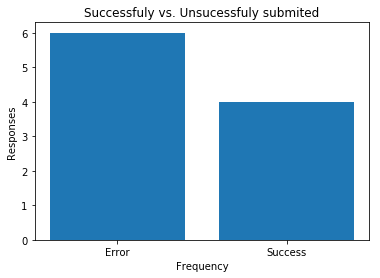
\includegraphics[scale = 0.90]{stat.png}
  \caption*{Successful vs. Unsuccessful}
  \label{fig:sincosine}
  \end{center}  
\end{figure}

\begin{figure}[h]
  \begin{center}
  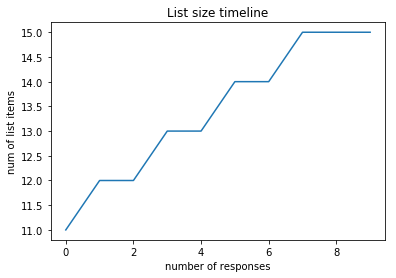
\includegraphics[scale = 0.90]{list_size_timeline.png}
  \caption*{Populating Entries}
  \label{fig:sincosine}
  \end{center}  
\end{figure}
%solution-end

\subsection*{Output - from the server}
%solution-start
\begin{verbatim}
127.0.0.1:50142 - - [08/Nov/2017 11:35:39] "HTTP/1.1 POST /form" - 200 OK
127.0.0.1:50144 - - [08/Nov/2017 11:35:39] "HTTP/1.1 POST /form" - 200 OK
127.0.0.1:50146 - - [08/Nov/2017 11:35:39] "HTTP/1.1 POST /form" - 200 OK
127.0.0.1:50148 - - [08/Nov/2017 11:35:39] "HTTP/1.1 POST /form" - 200 OK
127.0.0.1:50150 - - [08/Nov/2017 11:35:39] "HTTP/1.1 POST /form" - 200 OK
127.0.0.1:50152 - - [08/Nov/2017 11:35:39] "HTTP/1.1 POST /form" - 200 OK
127.0.0.1:50155 - - [08/Nov/2017 11:35:39] "HTTP/1.1 POST /form" - 200 OK
127.0.0.1:50157 - - [08/Nov/2017 11:35:39] "HTTP/1.1 POST /form" - 200 OK
127.0.0.1:50159 - - [08/Nov/2017 11:35:39] "HTTP/1.1 POST /form" - 200 OK
127.0.0.1:50161 - - [08/Nov/2017 11:35:39] "HTTP/1.1 POST /form" - 200 OK
127.0.0.1:50163 - - [08/Nov/2017 11:35:39] "HTTP/1.1 POST /form" - 200 OK
127.0.0.1:50165 - - [08/Nov/2017 11:35:39] "HTTP/1.1 POST /form" - 200 OK
127.0.0.1:50167 - - [08/Nov/2017 11:35:39] "HTTP/1.1 POST /form" - 200 OK
127.0.0.1:50169 - - [08/Nov/2017 11:35:39] "HTTP/1.1 POST /form" - 200 OK
\end{verbatim}
%solution-end
%-------------------------------------------------------------------------------

\makefooter

\end{document}

